\chapter[Mixed Formulation]{Mixed formulation}
\label{chap:MixedFormulation}
\begin{chapabstract}
    This chapter investigates the implementation of a mixed formulation in the HiDeNN framework.
\end{chapabstract}

\minitoc

\section{Element wise architecture}

When moving from linear 1D elements to higher order or dimensions, the use of an element wise architecture appears more versatile. The shape functions are therefore built on each element as opposed to globally on the mesh. 

One way of combining those approaches would be to add an \emph{Assembly layer} layer before the interpolation layer that rebuilds the global shape functions at the structure's (mesh) scale.

For each element, a sub-neural network would be built so that the output consists on the local shape functions $\Tilde{N}_i$ defined on the element. 

\Rq{At this point, several versions of the same shape function (associated to the same node) can exist independently through different elements.}

The \emph{Assembly layer} layer would then reconnect every local version $\Tilde{N}_i$ of a given global shape function $N_i$ associated to the $i-\text{th}$ node of the mesh. This layer would be a linear layer (without bias) that inputs all the $\Tilde{N}_i$ and outputs a smaller layer of the $N_i$.
The weight matrix of such a layer would read
\begin{equation}
    w_{i,d\left(e-1\right)+k} = \begin{cases}
        1,\text{ if }k-\text{th node of element }e\text{ is node }i \\
        0,\text{ otherwise}
    \end{cases}
\end{equation}

\section{Continuous vs. Discontinuous global shape functions}

Contrary to what we though, we in fact need to use the "leaking" version of shape functions (see \cref{fig:Continuous}). This might complicate the composition of global shape functions in higher dimensions, as the problem of non-zero values outside given element can not be simply solved by subtracting a constant value. However, creating the discontinuous global shape functions (see \cref{fig:Discontinuous}) is not possible using differentiable functions.

 We might still consider using the filter in front of the neural network: for $x \neq x_i$, $u(x)$ is obtained by interpolation provided by the neural network; for $x \neq x_i$, $u(x)$ is obtained directly as $u_i$. This is not necessary to deal with the incorrect value of shape functions, but it wold help us avoid the problem with zero derivatives.

 
\begin{figure}
    \centering
    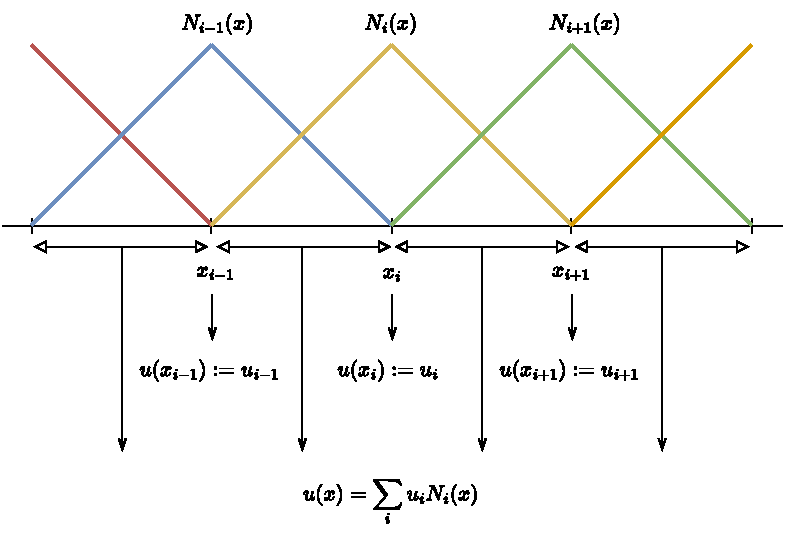
\includegraphics[trim={0 0 0 0},clip,width = 0.6\linewidth]{Figures/ShapeFunctions_1.drawio.pdf}    
    \caption{Treatment of points where the value of shape function is not defined correctly. }
    \label{fig:ShFDiscont}
\end{figure}


\section{Miscellaneous}

\Rq{In the mixed formulation, prescribing Neumann boundary conditions would be the same as imposing "Dirichlet boundary conditions" on the derivative field. It each space (primal and dual) the boundary conditions would be strictly prescribed, only the link between the primal and dual quantity would be weakly constrained through the loss.}

\Rq{Could have a hybrid training using both intergaral and mixed formulation ? To have a indicator of error on the integral versino aswell ?}
 
% \begin{figure}
%     \centering
%     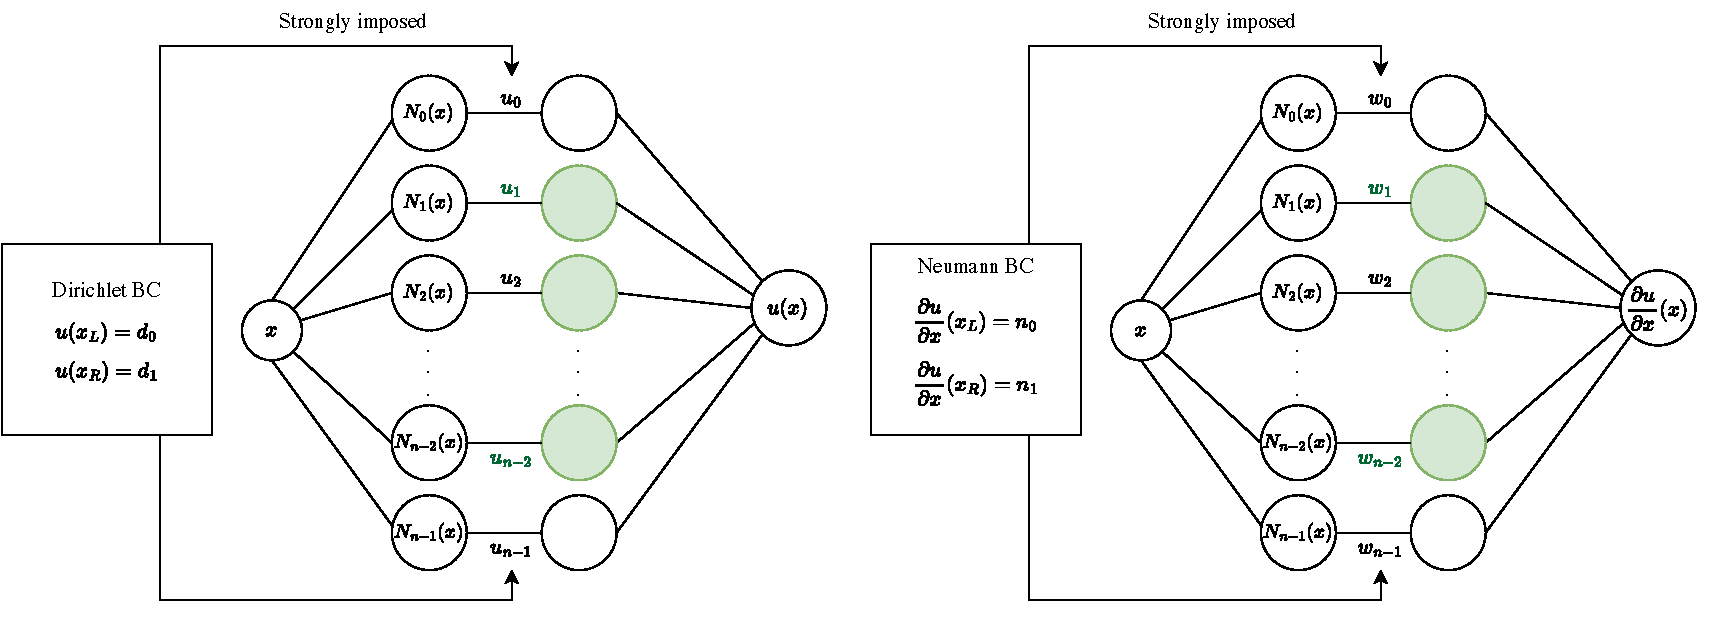
\includegraphics[trim={0 0 0 0},clip,width = 0.95\linewidth]{Figures/BC.drawio.pdf}    
%     \caption{Strong imposition of Dirichlet and Neumann boundary conditions in the associated NN.  }
%     \label{fig:ShFDiscont}
% \end{figure}

\begin{figure}
    \centering
    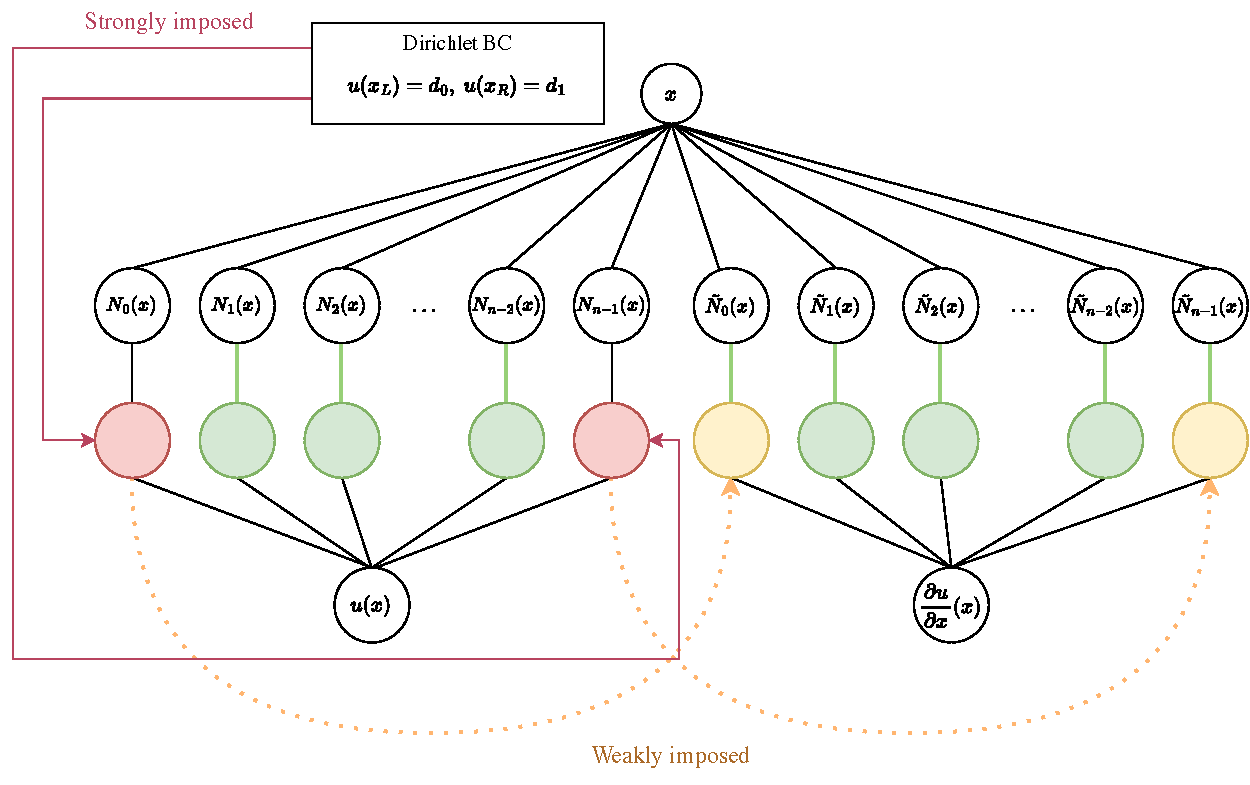
\includegraphics[trim={0 0 0 0},clip,width = 0.9\linewidth]{Figures/BC_1.drawio.pdf}    
    \caption{Neural network representation of mixed formulation for problem with Dirichlet boundary conditions. The boundary conditions are strictly prescribed for the NN providing the prediction of displacement $u$ and weakly (through loss function) for the NN providing the prediction of derivative of displacement $\frac{\partial u}{\partial x}$.   }
    \label{fig:BCsMixed}
\end{figure}


\section{Neumann boundary conditions}

With the mixed formulation an important question concern the way boundary conditions are prescribed.

They can be seen as Dirichlet boundary conditions on the dual field, \emph{i.e.} constraints in the interpolation. A difficulty may arise when we want to implement relation constraints between different components. Indeed, in such a case the components are still free to evolve but under a given constraint.

Such a constraint can then be prescribed before evaluating the NN within the training loop so that it would be updated as the stress nodal quantities evolve as illustrated in \cref{alg:NeumannBCs}.



\RestyleAlgo{ruled}

%% This is needed if you want to add comments in
%% your algorithm with \Comment
\SetKwComment{Comment}{/* }{ */}
\SetEndCharOfAlgoLine{}
\begin{algorithm}[hbtp!]
	\caption{Prescribing Neumann boundary conditions during training}\label{alg:NeumannBCs}
	\textbf{Inputs: } \code{model\_stress}, \code{model\_disp}, \code{\{$\sigma_i$\}}, \code{\{$u_i$\}} \textcolor{GreenLMS}{\Comment*[r]{Two models and corresponding nodal quantities}}
	
	\While(\textcolor{GreenLMS}{\Comment*[r]{\hspace{-5pt}Training loop \hspace{-6pt}}}){Training}{
		Compute the $\vect{n}\text{ on }\partial \Omega$ \textcolor{GreenLMS}{\Comment*[r]{ Update the normal vectors on the BCs}}
		
		 \code{\{$\sigma_i$\}} $ = f$( \code{\{$\sigma_i$\}}, \code{\{$u_i$\}}, $\vect{n}$)  \textcolor{GreenLMS}{\Comment*[r]{ Boundary conditions constraints}}
		 
		 $\sigm \left(\vect{x} \right) = $  \code{model\_stress}$\left(\vect{x} \right)$ \textcolor{GreenLMS}{\Comment*[r]{ Stress evaluation}}
		 
		 $\vect{u} \left(\vect{x} \right) = $  \code{model\_disp}$\left(\vect{x} \right)$    \textcolor{GreenLMS}{\Comment*[r]{ Displacement evaluation}}
		 
		 $\mathcal{L} = \mathcal{L}\left(\sigm \left(\vect{x} \right) , \vect{u} \left(\vect{x} \right)  \right)$  \textcolor{GreenLMS}{\Comment*[r]{ Loss evaluation}}

		\code{optimiser.step}  \textcolor{GreenLMS}{\Comment*[r]{ Update the models}}

	}
\end{algorithm}
\newpage
\Rqs{The evlaluation of the stress is then done using nodale stress values in the \code{model\_stress} that are consistant with the boundary conditions.}{Such an implementation would also easily allow dealing with changing normal during training for large strains for instance.}